\documentclass[11pt, twocolumn]{article}
\usepackage[utf8]{inputenc}
\usepackage[english]{babel}

\usepackage{multicol}

\usepackage[a4paper, margin=20mm]
{geometry} 
\usepackage[T1]{fontenc}
\usepackage[english]{babel}
\usepackage[utf8]{inputenc}
\usepackage{graphicx}
\usepackage[colorinlistoftodos]{todonotes}
\usepackage{booktabs}
\usepackage{multirow}
\providecommand{\com}[1]{\textit{\textbf{#1}}}
\usepackage{amsmath}
\usepackage{amsfonts}
\usepackage{amssymb}
\usepackage{graphicx}
\usepackage{float}
\usepackage{multirow}
\usepackage{colortbl}
\usepackage[utf8]{inputenc}
\usepackage{appendix}
\usepackage[mathscr]{euscript}
\usepackage{mathabx}
\usepackage{physics}
\usepackage{bbold}
\usepackage{bm}
\usepackage{subcaption}
\usepackage{wrapfig}

\usepackage{enumerate}

\newtheorem{teo}{Theorem}[section]
\newtheorem{prop}[teo]{Proposition}

% \theoremstyle{definition}
\newtheorem{lema}[teo]{Lemma}
\newtheorem{defi}[teo]{Definition}
\newtheorem{ej}[teo]{Example}
\newtheorem{obs}[teo]{Remark}
\newtheorem{cor}[teo]{Corollary}

\usepackage{hyperref}

\usepackage{amssymb}% 
\usepackage{pifont}%
\newcommand{\xmark}{\ding{54}}%


\usepackage{multicol}
\title{Hardware-efficient variational quantum eigensolver \\with entangled measurements}
\date{June 2021}
\author{Francisco Escudero, David Fernández, Gabriel Jaumà, Guillermo F. Peñas, Luciano Pereira}
\begin{document}
% \begin{multicols}
\maketitle

%\section{Introduction}

\section{Introduction.}
The variational quantum eigensolver (VQE) \cite{peruzzo2014variational} is a hybrid quantum-classical algorithm whose aim is to find the ground state of a Hamiltonian in near intermediate-scale quantum (NISQ) devices \cite{NISQ}. VQE starts by mapping the Hamiltonian into qubits operators. A variational quantum circuit is chosen to transform an initial state into a trial ground state. The energy of the trial state is estimated in the quantum computer according to the Hamiltonian. Finally, a classical optimizer receives the variational parameters and the energy of the trial state, and suggests a new set of parameters that might produce a ground state with a lower energy. To ensure an optimal operation, each of these steps must be efficient and tailored for a specific problem. 

Despite the great advances made in recent years, implementing VQE is still challenging. On the one hand, current devices have short coherence times, thus, only low-depth circuits are implemented with high quality \cite{kandala2017hardware}. On the other hand, the number of measurements required to evaluate the energy is extremely large for quantum applications \cite{Wecker2015}. For example, obtaining the energy of the molecule LiH requires the measure of 631 different Pauli observables. 

Both problems have been studied independently. The first one can be handled employing hardware-efficient circuits \cite{kandala2017hardware}, which take advantage of entanglement between neighboring qubits according to the device’s architecture. For the second problem, the number of required observables can be reduced by jointly measuring compatible Pauli strings  in Entangled Measurements (EM) \cite{hamamura2020efficient}. In this project, we tackle both obstacles simultaneously using Hardware-Efficient Entangled Measurements (HEEM), which are measurements that only use entanglement between neighboring qubits. The use of HEEM reduces the number of measurements needed to perform VQE without compromising the quality of the experiment. 

\begin{table}
\resizebox{\columnwidth}{!}{
\begin{tabular}{c|cccccccc|c|}
\cline{2-10}
                          & \multicolumn{1}{c|}{$XX$} & \multicolumn{1}{c|}{$YZ$}       & \multicolumn{1}{c|}{$ZY$}       & \multicolumn{1}{c|}{$YY$}                  & \multicolumn{1}{c|}{$XZ$}                  & \multicolumn{1}{c|}{$ZX$}                  & \multicolumn{1}{c|}{$ZZ$}                  & $XY$                  & $YX$                  \\ \hline
\multicolumn{1}{|c|}{$XX$} & \multicolumn{1}{c|}{---}  & \multicolumn{1}{c|}{$\Omega^X$} & \multicolumn{1}{c|}{$\Omega^X$} & \multicolumn{1}{c|}{Bell}                  & \multicolumn{1}{c|}{\xmark} & \multicolumn{1}{c|}{\xmark} & \multicolumn{1}{c|}{Bell}                  & \xmark & \xmark \\ \hline
\multicolumn{1}{|c|}{$YZ$} & \multicolumn{1}{c|}{}     & \multicolumn{1}{c|}{---}        & \multicolumn{1}{c|}{$\Omega^X$} & \multicolumn{1}{c|}{\xmark} & \multicolumn{1}{c|}{\xmark} & \multicolumn{1}{c|}{$\chi$}                & \multicolumn{1}{c|}{\xmark} & $\chi$                & \xmark \\ \cline{1-1} \cline{3-10} 
\multicolumn{1}{|c|}{$ZY$} &                           & \multicolumn{1}{c|}{}           & \multicolumn{1}{c|}{---}        & \multicolumn{1}{c|}{\xmark} & \multicolumn{1}{c|}{$\chi'$}               & \multicolumn{1}{c|}{\xmark} & \multicolumn{1}{c|}{\xmark} & \xmark & $\chi'$               \\ \cline{1-1} \cline{4-10} 
\multicolumn{1}{|c|}{$YY$} &                           &                                 & \multicolumn{1}{c|}{}           & \multicolumn{1}{c|}{---}                   & \multicolumn{1}{c|}{$\Omega^Y$}            & \multicolumn{1}{c|}{$\Omega^Y$}            & \multicolumn{1}{c|}{Bell}                  & \xmark & \xmark \\ \cline{1-1} \cline{5-10} 
\multicolumn{1}{|c|}{$XZ$} &                           &                                 &                                 & \multicolumn{1}{c|}{}                      & \multicolumn{1}{c|}{---}                   & \multicolumn{1}{c|}{$\Omega^Y$}            & \multicolumn{1}{c|}{\xmark} & \xmark & $\chi'$               \\ \cline{1-1} \cline{6-10} 
\multicolumn{1}{|c|}{$ZX$} &                           &                                 &                                 &                                            & \multicolumn{1}{c|}{}                      & \multicolumn{1}{c|}{---}                   & \multicolumn{1}{c|}{\xmark} & $\chi$                & \xmark \\ \cline{1-1} \cline{7-10} 
\multicolumn{1}{|c|}{$ZZ$} &                           &                                 &                                 &                                            &                                            & \multicolumn{1}{c|}{}                      & \multicolumn{1}{c|}{---}                   & $\Omega^Z$            & $\Omega^Z$            \\ \cline{1-1} \cline{8-10} 
\multicolumn{1}{|c|}{$XY$} &                           &                                 &                                 &                                            &                                            &                                            & \multicolumn{1}{c|}{}                      & ---                   & $\Omega^Z$            \\ \cline{1-1} \cline{9-10} 
\multicolumn{1}{|c|}{$YX$} &                           &                                 &                                 &                                            &                                            &                                            &                                            &                       & ---                   \\ \cline{1-1} \cline{10-10} \hline  
\end{tabular}}
\caption{Compatibility relation between two-qubits Pauli strings. The \xmark\ indicates that the corresponding Pauli strings are not jointly measurable. The other boxes contain the measurements that are compatible with the corresponding Pauli strings.}
\label{table1}
\end{table}


\section{Hardware-efficient grouping}

Consider a Hamiltonian $H$ whose decomposition in terms of Pauli strings is
\begin{align}\label{eq1}
    H =\sum_i h_i P_i\,,
\end{align}
where $P_i$ are tensor products of Pauli operators ($X,Y,Z$) and the identity ($I$). The most naive routines used to compute the expected value of H require measuring each Pauli string $P_i$ separately. Each measurement is performed with a Tensor Product Basis (TPB), which are the tensor products of the bases $\{\mathcal{X},\mathcal{Y},\mathcal{Z}\}$, where $\mathcal{X}=\{\ket{0}\pm\ket{1}\}$, $\mathcal{Y}=\{\ket{0}\pm i\ket{1}\}$, and  $\mathcal{Z}=\{\ket{0},\ket{1}\}$. 

This strategy can be improved. As several Pauli string are compatible with the same TPB (for instance, $XIZ$ and $XYZ$ are compatible with $\mathcal{X}\otimes\mathcal{Y}\otimes\mathcal{Z}$), the same measurement can be used for computing the expected values of more than one Pauli strings. This way, we can make groups of Pauli strings that are compatible with the same TPB, and perform a measurement for each group.
This grouping strategy can go further, and more complex and profitable strategies can be constructed using entanglement. 

\pagebreak
\begin{table}[]
\resizebox{8.5cm}{!}{
\begin{tabular}{c|c|c|c|c|c|}
\cline{2-6}
                             & \multicolumn{1}{l|}{qubits} & \multicolumn{1}{l|}{No grouping} & \multicolumn{1}{l|}{TPB} & \multicolumn{1}{l|}{EM}  & \multicolumn{1}{l|}{HEEM} \\ \hline
\multicolumn{1}{|l|}{H$_2$}  &   4                          & 15                               & 5                        & 2                               & 2 \\ \hline
\multicolumn{1}{|l|}{LiH*}   &   4                         & 100                              & 25                        & 9                              & 9 \\ \hline
\multicolumn{1}{|l|}{LiH}     &  12                          & 631                              & 136                        & 38                              & 94 \\ \hline
\multicolumn{1}{|l|}{BeH$_2$*}&  7                           & 545                              & 121                      & 74                              & 103 \\ \hline
\multicolumn{1}{|l|}{BeH$_2$} &  14                          & 666                              & 140                      & 41                              & 110 \\ \hline
\multicolumn{1}{|l|}{H$_2$O}  &  14                           & 1086                             & 224                      & 58                              & 146 \\ \hline

\end{tabular}
}
\caption{ Number of groups for some molecules using different grouping strategies. HEEM groups have been obtained respecting the connectivity of the quantum device \emph{ibmq\_paris}. The EM and HEEM are results of 200 random sorting of the Pauli strings. LiH* and BeH$_2$* has qubit reduction.}
\label{table2}
\end{table}

\pagebreak For example, the Pauli strings $ZY$, $XZ$ and $YX$ are simultaneously measurable in the entangled basis 
\begin{align} \label{chitilde}
    \chi'=\{& \mp|00\rangle+i|01\rangle\pm|10\rangle+i|11\rangle,\\ \nonumber
            & i|00\rangle \pm|01\rangle +i|10\rangle \mp |11\rangle \}. 
\end{align}

\noindent With a wider range of EM, as the ones shown in \cite{hamamura2020efficient}, one can establish the following general strategy:
\begin{enumerate}
    \item Define a set of admissible measurements $E$.\label{step1}
    \item Decompose $H$ in terms of Pauli strings.\label{step2}
    \item Make groups of $P_i$ that are jointly measurable in the same admissible basis. \label{step3}
    \item Measure the expected value of each group independently and then compute the expected value of $H$ using \eqref{eq1}.\label{step4}
\end{enumerate}
\noindent If only TPBs are considered as admissible, the standard technique to make the groups is by means of the Pauli graph and the Largest Degree First Coloring (LDFC) algorithm. This is the protocol currently followed in Qiskit \cite{QISKIT}. When more bases are considered in addition to TPB, the analogue of the Pauli graph is hard to build. Despite the fact that developing a perfect grouping algorithm is an NP-complete problem \cite{Coloring}, the LDFC strategy can be improved. For these reasons, in \cite{hamamura2020efficient} the authors propose an alternative algorithm to do the grouping with entangled bases. 

 We have developed a Python library \cite{github}, based on the grouping algorithm presented in \cite{hamamura2020efficient}. This algorithm groups the Pauli strings using the following set of admissible measurements: TPBs, the two-qubit entangled basis introduced in \cite{hamamura2020efficient} (Bell, $\Omega^X$, $\Omega^Y$, $\Omega^Z$ and $\chi$), and the basis $\chi'$. Basis $\chi'$ was introduced by us to complete table \ref{table1}, ensuring that every pair of compatible two-qubit Pauli strings can be measured with one entangled basis. Furthermore, to implement HEEM we have adapted the grouping algorithm to consider as admissible measurements only those which entangle qubits that are physically connected in the device.
   
We show in table \ref{table2} the number of groups obtained with our algorithm for the Hamiltonians of several molecules. We can see that grouping with EM and HEEM reduces the number of groups obtained via TPBs. We found that the number of groups by HEEM ranges between the values given by TPB and EM. This is reasonable, since HEEM is restricted by the connectivity of the quantum device and EM not. Coincidentally, the best grouping for LiH* respects the device's architecture, thus, HEEM and EM obtain the same groups.

%%%%%%%%%%%%%%%%%%%%%%%%%%%%%%%%%%%%%%%%%%%%%%%
\begin{figure}[b!]
    \centering
    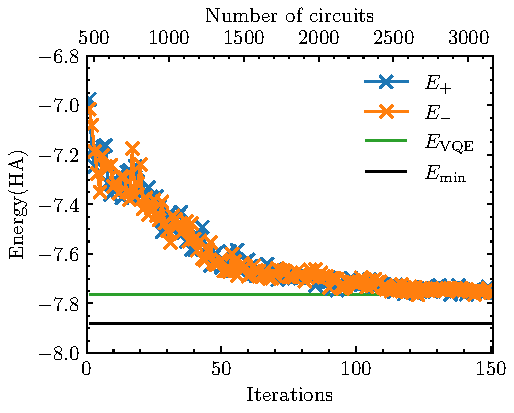
\includegraphics[width=0.95\linewidth]{Experiment.pdf}
    \caption{Experimental results of VQE for the 4-qubits LiH Hamiltonian for $d=1.54$\r{A}. The experiment was conducted in the device \emph{ibmq\_guadalupe}. The classical optimizer used was SPSA with 150 iterations and calibrated with 50 function evaluations. Each circuit was evaluated with $2^{13}$ shots.}
    \label{fig:experiment}
\end{figure}
%%%%%%%%%%%%%%%%%%%%%%%%%%%%%%%%%%%%%%%%%%%%%%

\section{Simulations and Experiment}
We have solved experimentally the lowest energy state of the LiH molecule by VQE with HEEM in the IBM quantum device \emph{ibmq\_guadalupe}, see Fig.~\ref{fig:experiment}. Each energy estimation required measuring $9$ HEEMs. Since the classical optimization required $351$ energy measurements, the total number of circuits used was $3159$. We have obtained a relative error of $0.015$ Ha, which is very similar to that obtained by \cite{kandala2017hardware}, where the LiH was solved using TPBs. In their experiment, each energy evaluation required the measurement of $25$ TPBs, which after 351 energy evaluation leads to a total of $8775$ circuits. As it can be seen, we obtain a similar value for the energy at the same number of iterations, but employing about a third of their number of circuits.

We have also studied the molecule of ${\rm BeH_2}$ simulating a noisy quantum computer, see Fig. \ref{fig:simulation}. We observe a significant noise suppression when comparing HEEM with EM due to the reduction of noisy two-qubit gates. As in the experimental case, we observe that HEEM and TPB have a very similar performance regarding noise and convergence value, whereas HEEM converges with a lower number of circuits.

\section{Conclusions and Outlook}
In this project, we have constructed a Qiskit-based library to execute the VQE algorithm with HEEM \cite{github}. These are measurements that take advantage of entanglement between neighboring qubits, respecting the architecture of the chip so that they can be efficiently implemented in NISQ devices. We provide a method for creating groups of Pauli strings that are compatible by HEEM. We show that grouping by HEEM leads to a reduction in the number of measurements needed to evaluate the energy for a variety of molecules. We have carried out numerical simulations of $\text{BeH}_2$, achieving a significant noise and circuit reduction with HEEM. Moreover, we have experimentally solved the LiH molecule, obtaining results comparable with previous research but with a smaller number of circuits. Our results are promising, suggesting that HEEM reduces the number of measurements required for VQE without compromising the fidelity of the experiment. We expect that our contributions will expand the range of simulable systems in current NISQ devices. 

We have encountered a rich variety of phenomena related to the project that are worth exploring in the future. Firstly, the grouping algorithm used is highly dependent on the order chosen to map the qubits of the Hamiltonian to the qubits of the chip, as well as on the order in which the measurements are assigned to the groups (in the algorithm one can choose which measurements will be preferentially assigned). Considering this, we will investigate how to obtain an optimal ordering strategy. Secondly, will search for good \textit{universal groupings}. For each size of Pauli strings $N$ one can consider the worst case scenario: an observable including the $4^N$ possible strings. The groups done for this case would work for any observable of $N$ qubits, in that sense they would be \textit{universal}. With them one can create a database with groups valid for every observable of a given size $N$. Thirdly, we plan to consider entangled-measurements involving 3 (or more) qubits, i.e., we will reproduce table \ref{table1} for 3 (or more) qubits and update our library with those measurements. Finally, we expect to perform numerical simulations and experiments for larger molecules, such as ${\rm BeH_2}$ and ${\rm H_2O}$.\\


%%%%%%%%%%%%%%%%%%%%%%%%%%%%%%%%%%%%%%%%%
\begin{figure}[H]
    \centering
    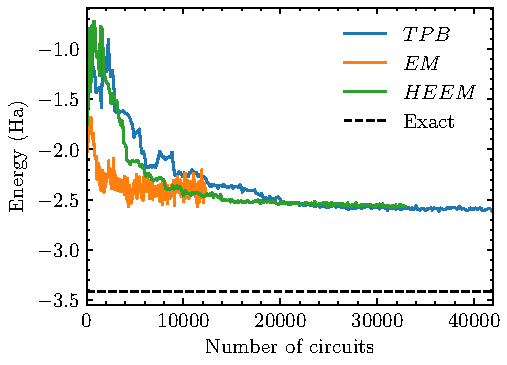
\includegraphics[width=0.95\linewidth]{simulation_BeH.pdf}
    \caption{ Numerical results of VQE for the 7-qubits ${\rm BeH_2}$ Hamiltonian for $d=1.34$\r{A}. The simulations where done considering the noise and the connectivity of the device \emph{ibmq\_16\_melbourne}. The classical optimizer used was SPSA with 300 iterations and calibrated with 50 function evaluations. Each circuit was evaluated with $2^{13}$ shots.}
    \label{fig:simulation}
\end{figure}
%%%%%%%%%%%%%%%%%%%%%%%%%%%%%%%%%%%%%%%%%

\section{Contributions}
FE developed the grouping algorithm. DF, LP, and GP developed the VQE class. GJ and DF performed the simulations. LP performed the experiment. GJ found the entangled basis $\chi'$. All authors contributed equally to the writing of the report and the recording of the video. 

\bibliographystyle{unsrt}
\bibliography{Bibliography}
\end{document}
